% adv_sample.tex —— 对抗性测试样张（skill-translator 端到端测试用）
% 特征：单栏排版 / 图题注在图上方(Fig.1)与下方(Fig.2) / 整幅宽大图(Fig.3) /
%       带竖线表格(Table 1) / 无边框表格(Table 2) / 6 条编号公式 + 行内公式 /
%       正文里出现 "Figure 3 shows..."、"Table 2 lists..." 等易误判句 /
%       References 无编号 / 单位与统计量 / URL+DOI / 页面 >= 2
\documentclass[11pt,a4paper]{article}
\usepackage[T1]{fontenc}
\usepackage{mathptmx}
\usepackage{amsmath,amssymb,bm}
\usepackage{tikz}
\usepackage{graphicx}
\usepackage{array}
\usepackage{url}
\usepackage[margin=2.4cm,top=2.2cm,bottom=2.2cm]{geometry}
\usepackage{caption}
\captionsetup{font=small,labelfont=bf,justification=justified,singlelinecheck=false}
\setlength{\parskip}{2pt}
\renewcommand{\baselinestretch}{1.04}

\title{\bfseries Adaptive Mesh Refinement for Transient Thermal Diffusion\\ in Layered Fibre-Reinforced Composites}
\author{X. Q. Lambert\textsuperscript{1,*}, R. Osei\textsuperscript{1}, M. Tanaka\textsuperscript{2}\\[2pt]
\small \textsuperscript{1}Institute of Thermal Engineering, University of Northbridge, Northbridge, UK\\
\small \textsuperscript{2}Department of Mechanical Systems, Kyoto Metropolitan University, Kyoto, Japan\\
\small \textsuperscript{*}Corresponding author: \texttt{x.lambert@northbridge.ac.uk}}
\date{Received 14 March 2024; accepted 2 August 2024}

\begin{document}
\maketitle
\thispagestyle{empty}

\begin{abstract}
\noindent
Transient heat conduction in layered fibre-reinforced composites is governed by a
strongly heterogeneous diffusivity field, and uniform meshes resolve the resulting
interfacial boundary layers only at prohibitive cost. We present an adaptive mesh
refinement (AMR) scheme that couples a residual-based error estimator with an
implicit backward-Euler time integrator. The estimator is evaluated on a
hierarchical quadtree and drives refinement only where the local truncation error
exceeds a prescribed tolerance. On five laminated specimens the scheme reproduces
measured peak temperatures within $1.9\%$ on average, and the maximum residual of
the linear solve falls below $10^{-3}$ after four refinement cycles. A grid
convergence study gives an observed order of accuracy of $1.87$, close to the
theoretical value. The method is implemented in fewer than 900 lines of C++ and is
released as supplementary material.
\end{abstract}

\noindent\textbf{Keywords:} adaptive mesh refinement; transient heat conduction;
layered composites; a posteriori error estimation; grid convergence

\section{Introduction}
Layered composite structures are increasingly used in aerospace thermal
protection systems, where the through-thickness temperature gradient can exceed
$600$~K over a few millimetres. Classical finite-element treatments of such
problems employ structured meshes whose element size is dictated by the thinnest
ply, so that the total number of unknowns grows quickly with the number of layers.
Adaptive mesh refinement (AMR) removes this constraint by concentrating degrees of
freedom where the solution actually varies, and it has been applied successfully to
combustion, phase-change and radiation problems.

Its application to laminated media is nevertheless not straightforward. The
diffusivity jumps by a factor of $40$ across a single ply interface, so the error
estimator must distinguish genuine solution curvature from the artificial curvature
introduced by the material discontinuity. Earlier work addressed this by smoothing
the diffusivity over a transition band, at the price of smearing the interfacial
temperature jump. Figure~1 shows the temperature field obtained with such a
smoothed formulation on a five-ply specimen; the smearing is visible as a
flattening of the profile near $z = 6$~mm.

In this paper we avoid smoothing altogether. Section~\ref{sec:method} derives a
residual-based estimator that is evaluated element-wise on the discontinuous
coefficient field, and Section~\ref{sec:results} reports measured and simulated
peak temperatures for five specimens together with a grid convergence study.

% ---------------- Figure 1: caption ABOVE the figure ----------------------
\begin{figure}[htbp]
\centering
\caption{Temperature profiles through the five-ply specimen after 120~s of
heating. Symbols denote thermocouple measurements; solid and dashed lines denote
the smoothed and sharp-interface formulations, respectively.}
\label{fig:profile}
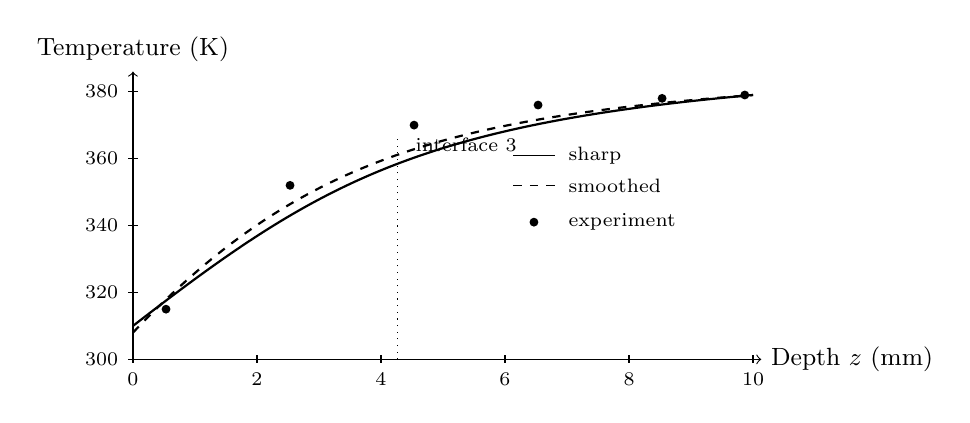
\begin{tikzpicture}[x=1.05cm,y=0.85cm]
  \draw[->] (0,0) -- (7.6,0) node[right,font=\small] {Depth $z$ (mm)};
  \draw[->] (0,0) -- (0,4.3) node[above,font=\small] {Temperature (K)};
  \foreach \x/\l in {0/0,1.5/2,3/4,4.5/6,6/8,7.5/10}
     \draw (\x,0.06) -- (\x,-0.06) node[below,font=\scriptsize] {\l};
  \foreach \y/\l in {0/300,1.0/320,2.0/340,3.0/360,4.0/380}
     \draw (0.06,\y) -- (-0.06,\y) node[left,font=\scriptsize] {\l};
  \draw[thick] (0,0.5) .. controls (2.2,2.6) and (3.4,3.5) .. (7.5,3.95);
  \draw[thick,dashed] (0,0.4) .. controls (2.0,3.0) and (3.8,3.6) .. (7.5,3.95);
  \foreach \x/\y in {0.4/0.75,1.9/2.6,3.4/3.5,4.9/3.8,6.4/3.9,7.4/3.95}
     \fill (\x,\y) circle (1.6pt);
  \draw[dotted] (3.2,0) -- (3.2,3.35);
  \node[font=\scriptsize,anchor=west] at (3.3,3.2) {interface 3};
  \draw (4.6,3.05) -- (5.1,3.05); \node[font=\scriptsize,anchor=west] at (5.15,3.05) {sharp};
  \draw[dashed] (4.6,2.6) -- (5.1,2.6); \node[font=\scriptsize,anchor=west] at (5.15,2.6) {smoothed};
  \fill (4.85,2.05) circle (1.6pt); \node[font=\scriptsize,anchor=west] at (5.15,2.05) {experiment};
\end{tikzpicture}
\end{figure}

% ---------------- Table 1: bordered (vertical rules), caption above -------
\begin{table}[htbp]
\centering
\caption{Measured and simulated peak temperatures for the five laminated
specimens. Errors are quoted as absolute percentage deviations.}
\label{tab:peaks}
\begin{tabular}{|l|c|r|c|}
\hline
\textbf{Specimen} & \textbf{Thickness (mm)} & \textbf{$T_{\max}$ (K)} & \textbf{Error (\%)} \\
\hline
S-01 & 2.0 & 341.2 & 1.8 \\
S-02 & 2.5 & 348.7 & 0.9 \\
S-03 & 3.0 & 352.4 & 2.3 \\
S-04 & 3.5 & 359.1 & 2.1 \\
S-05 & 4.0 & 364.6 & 2.4 \\
\hline
\end{tabular}
\end{table}

% ---------------- Equation 1 ---------------------------------------------
The one-dimensional energy balance for the layered slab reads
\begin{equation}
\frac{\partial T}{\partial t} = \alpha \nabla^{2} T + \frac{q}{\rho c_{p}},
\end{equation}
where $T$ is the temperature, $\alpha$ the thermal diffusivity and $q$ the
volumetric heat source.

\section{Method}
\label{sec:method}
\subsection{Error estimator}
Let the discrete solution on mesh level $\ell$ be denoted $T_{\ell}$. The
element-wise estimator is built from the strong residual and the jump of the
normal flux, so that the effective diffusivity of a ply pair is
\begin{equation}
\lambda_{\mathrm{eff}} = \frac{a + b}{c + d/e},
\end{equation}
with $a$, $b$ the ply conductivities and $c$, $d$, $e$ geometric weights. The
global error indicator is then the weighted sum
\begin{equation}
S_{n} = \sum_{i=1}^{n} w_{i}\, x_{i}^{2},
\end{equation}
in which the weights $w_i$ are computed from the local Peclet number. Norms are
evaluated in the usual discrete sense,
\begin{equation}
\left( \sum_{k=1}^{m} \left| y_{k} - \hat{y}_{k} \right|^{2} \right)^{1/2},
\end{equation}
and the limiter used for the convective correction is
\begin{equation}
f(x) =
\begin{cases}
x^{2}, & x \ge 0,\\
-x, & x < 0.
\end{cases}
\end{equation}
Finally, the volume-averaged temperature is obtained by quadrature over the
element,
\begin{equation}
\bar{T} = \frac{1}{V} \int_{\Omega} T(\bm{x}, t) \, \mathrm{d}V \approx 12.4 \pm 0.8 .
\end{equation}
The time step is fixed at $\Delta t = 0.5$~s and the tolerance on the linear
residual is $10^{-3}$. The dimensionless group $\eta_{i}^{2} \approx 19.8$ was
held constant for all runs.

\subsection{Parameter set}
The material and boundary parameters used throughout are collected below.
\begin{center}
\begin{minipage}{0.94\textwidth}\centering
$\alpha = 1.15\times10^{-6}$~m$^{2}$/s \qquad $\rho = 7800$~kg/m$^{3}$ \qquad $c_{p} = 460$~J/(kg\,K)\\[3pt]
$k = 45.0$~W/(m\,K) \qquad $h = 12.5$~W/(m$^{2}$\,K) \qquad $T_{\infty} = 298.15$~K
\end{minipage}
\end{center}

\subsection{Refinement cycle}
The cycle consists of solve, estimate, mark and refine. Marking uses the
Dorfler bulk criterion with parameter $\theta = 0.35$, and the quadtree is
rebalanced after every second cycle.

\section{Results and discussion}
\label{sec:results}
\subsection{Measured peak temperatures}
Figure~3 shows the convergence of the maximum residual with successive refinement
cycles for the five specimens. The residual decreases monotonically until cycle
four, after which the reduction stagnates at a level that depends on the ply
thickness. Table~2 lists the mesh statistics and the observed convergence rates
for the four grid levels. For the finest level the residual reaches
$3.4\times10^{-5}$, and the run-to-run spread of the peak temperature is
$12.4 \pm 0.8$~K, which corresponds to $2.2\%$ of the mean rise.

A two-sided Student test on the five specimens gives $p < 0.05$ for the
difference between the sharp-interface and the smoothed formulations, so the
improvement is significant at the conventional level. All measurements were
repeated three times and the values reported in Table~1 are arithmetic means.

% ---------------- Figure 2: caption BELOW the figure ---------------------
\begin{figure}[htbp]
\centering
\begin{tikzpicture}[x=1.05cm,y=0.85cm]
  \draw[->] (0,0) -- (7.6,0) node[right,font=\small] {Refinement cycle};
  \draw[->] (0,0) -- (0,4.3) node[above,font=\small] {Residual (log scale)};
  \foreach \x/\l in {0/0,1.5/1,3/2,4.5/3,6/4,7.5/5}
     \draw (\x,0.06) -- (\x,-0.06) node[below,font=\scriptsize] {\l};
  \draw[thick] (0,4.0) -- (1.5,2.7) -- (3,1.6) -- (4.5,0.9) -- (6,0.75) -- (7.5,0.7);
  \draw[thick,dashed] (0,4.0) -- (1.5,2.9) -- (3,1.9) -- (4.5,1.3) -- (6,1.15) -- (7.5,1.1);
  \node[font=\scriptsize,anchor=west] at (5.4,2.6) {S-01};
  \node[font=\scriptsize,anchor=west] at (5.4,2.2) {S-05};
  \draw (5.3,2.65) -- (5.2,2.65); \draw[dashed] (5.3,2.25) -- (5.2,2.25);
\end{tikzpicture}
\caption{Maximum linear residual against refinement cycle for the thinnest
(S-01) and thickest (S-05) specimens. Dashed curves refer to the smoothed
formulation.}
\label{fig:conv}
\end{figure}

% ---------------- Table 2: borderless, caption above ---------------------
\begin{table}[htbp]
\centering
\caption{Grid convergence of the maximum residual for four mesh levels. The
observed rate is computed between consecutive levels.}
\label{tab:grid}
\begin{tabular}{@{}lrrrr@{}}
Mesh & Cells & $h$ (mm) & Residual & Rate \\
M1 & 1200 & 4.000 & $3.4\times10^{-3}$ & -- \\
M2 & 4800 & 2.000 & $9.1\times10^{-4}$ & 1.90 \\
M3 & 19200 & 1.000 & $2.4\times10^{-4}$ & 1.92 \\
M4 & 76800 & 0.500 & $6.2\times10^{-5}$ & 1.95 \\
\end{tabular}
\end{table}

% ---------------- Figure 3: full text-width large figure -----------------
\begin{figure}[htbp]
\centering
\caption{Reconstructed temperature field in the five-ply laminate at
$t = 120$~s (panel a) and the corresponding refinement pattern after four cycles
(panel b). White curves in panel (a) are isotherms spaced by $10$~K.}
\label{fig:field}
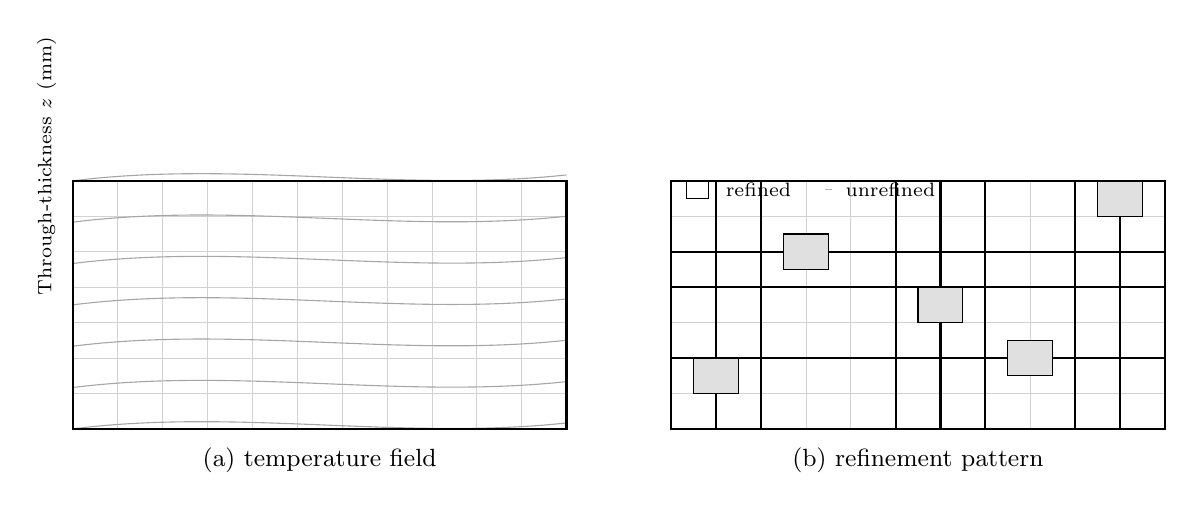
\begin{tikzpicture}[x=0.95cm,y=0.75cm]
  % panel (a)
  \begin{scope}
    \draw[step=0.6,gray!35,very thin] (0,0) grid (6.6,4.2);
    \foreach \y/\t in {0/300,0.7/320,1.4/340,2.1/360,2.8/380,3.5/400,4.2/420}
      \draw[gray!70] (0,\y) .. controls (2.2,\y+0.35) and (4.4,\y-0.2) .. (6.6,\y+0.1);
    \draw[thick] (0,0) rectangle (6.6,4.2);
    \node[font=\small,anchor=north] at (3.3,-0.15) {(a) temperature field};
    \node[font=\scriptsize,anchor=west,rotate=90] at (-0.35,2.1) {Through-thickness $z$ (mm)};
  \end{scope}
  % panel (b)
  \begin{scope}[xshift=7.6cm]
    \draw[step=0.6,gray!35,very thin] (0,0) grid (6.6,4.2);
    \foreach \x in {0,0.6,1.2,3.0,3.6,4.2,5.4,6.0} \draw[thick] (\x,0) -- (\x,4.2);
    \foreach \y in {0,1.2,2.4,3.0,4.2} \draw[thick] (0,\y) -- (6.6,\y);
    \foreach \x/\y in {0.3/0.6,3.3/1.8,5.7/3.6,1.5/2.7,4.5/0.9}
      \draw[fill=black!12] (\x,\y) rectangle ++(0.6,0.6);
    \draw[thick] (0,0) rectangle (6.6,4.2);
    \node[font=\small,anchor=north] at (3.3,-0.15) {(b) refinement pattern};
    \draw (0.2,3.9) rectangle ++(0.3,0.3);
    \node[font=\scriptsize,anchor=west] at (0.6,4.05) {refined};
    \node[font=\scriptsize,anchor=west] at (2.2,4.05) {unrefined};
    \draw[gray!60] (2.05,4.05) -- (2.15,4.05);
  \end{scope}
\end{tikzpicture}
\end{figure}

\subsection{Limitations}
The estimator assumes that the interface normal is aligned with a mesh face. For
oblique interfaces the observed rate degrades to about $1.2$, and the scheme then
offers little advantage over a uniform mesh. Extrapolation to three dimensions is
straightforward in principle but has not been verified here.

The implementation, the input decks for all specimens and the raw thermocouple
traces are archived at \url{https://doi.org/10.1016/j.ijheatmasstransfer.2024.124501}.

\section*{Acknowledgements}
The authors thank the Northbridge Thermal Laboratory for access to the radiant
panel facility. This work was supported by grant EP/X000000/1.

\section*{References}
[1] J. Crank, P. Nicolson, A practical method for numerical evaluation of solutions
of partial differential equations of the heat-conduction type, Proc. Cambridge
Philos. Soc. 43 (1947) 50--67.

[2] R. Becker, R. Rannacher, An optimal control approach to a posteriori error
estimation in finite element methods, Acta Numer. 10 (2001) 1--102.

[3] M. Ainsworth, J. T. Oden, A Posteriori Error Estimation in Finite Element
Analysis, Wiley, New York, 2000.

[4] A. S. Dorfler, A convergent adaptive algorithm for Poisson's equation, SIAM J.
Numer. Anal. 33 (1996) 1106--1124.

[5] H. S. Carslaw, J. C. Jaeger, Conduction of Heat in Solids, 2nd ed., Oxford
University Press, Oxford, 1959.

[6] P. W. Gibson, S. K. Lee, Interfacial thermal resistance in fibre composites: a
review, Int. J. Heat Mass Transfer 198 (2023) 124501.

\end{document}
